% filepath: /home/chen/Workspace/RISC_V/ZJU_CPU/pic/IFU/IFU.tex
\documentclass[tikz,border=2mm]{standalone}
\usetikzlibrary{shapes.geometric, arrows, positioning}

\tikzstyle{module} = [rectangle, rounded corners, minimum width=3cm, minimum height=1cm, text centered, draw=black, fill=blue!30]
\tikzstyle{signal} = [draw=black, -latex, thick]
\tikzstyle{topmodule} = [rectangle, rounded corners, draw=black, thick, minimum width=12cm, minimum height=10cm, text centered, dashed]

\begin{document}
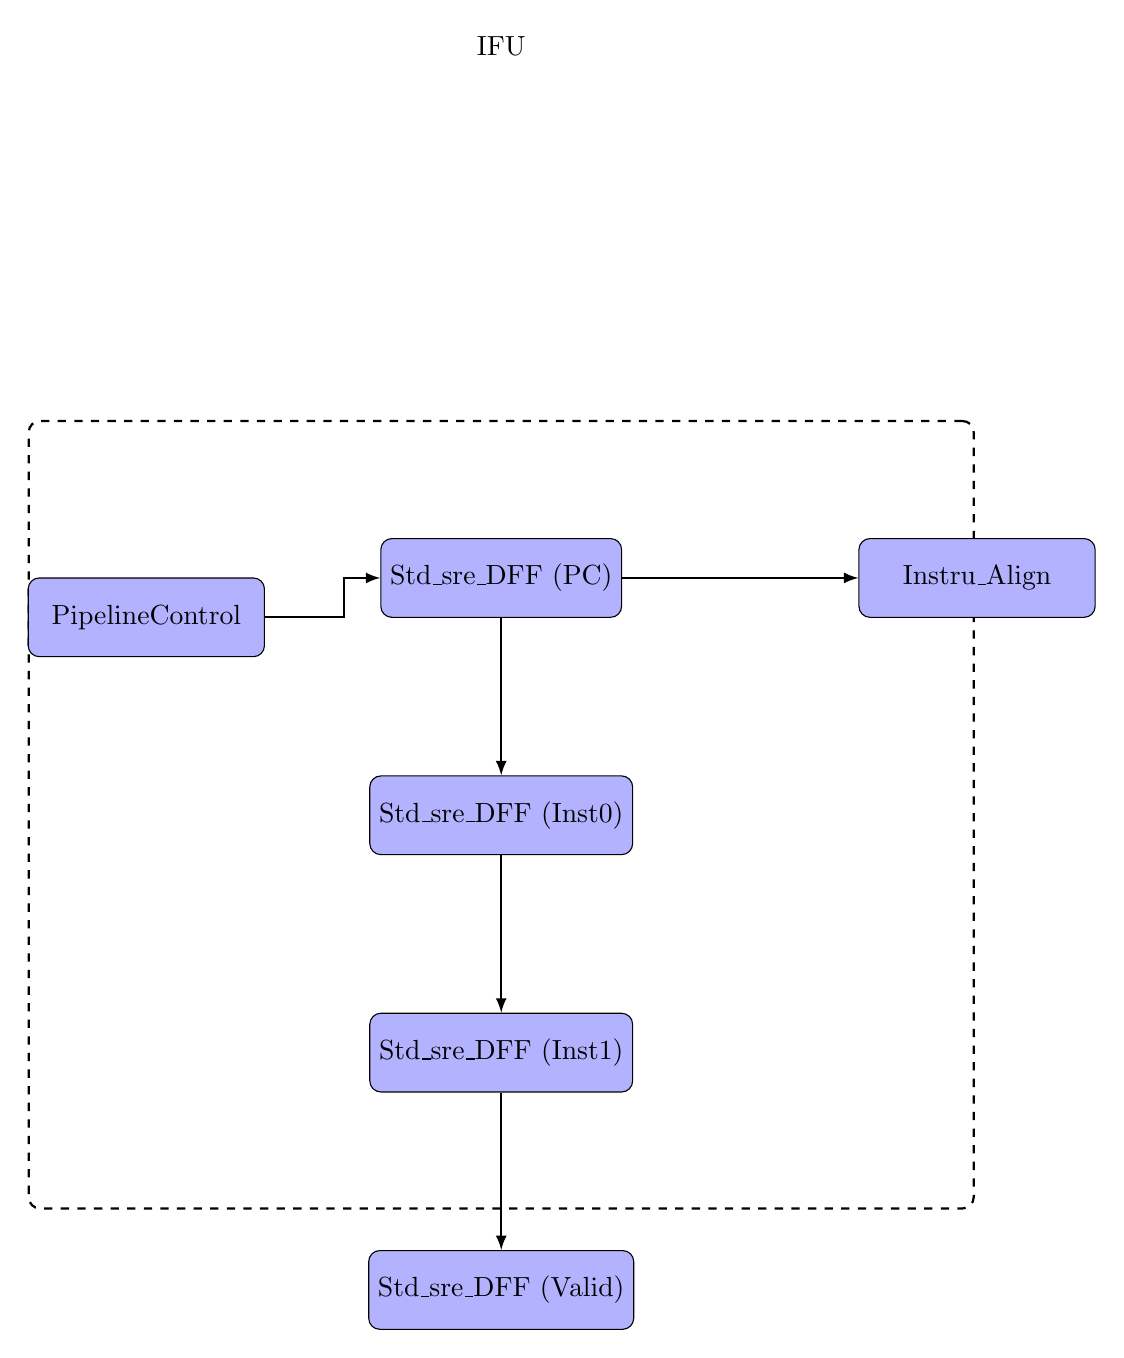
\begin{tikzpicture}[node distance=2cm]

% Top-level module (IFU)
\node (ifu) [topmodule, label={[yshift=4.5cm]IFU}] at (0, -4) {};

% Submodules inside IFU
\node (pipelinecontrol) [module, below left=2cm and 3cm of ifu.north] {PipelineControl};
\node (std_dff_pc) [module, below=1.5cm of ifu.north] {Std\_sre\_DFF (PC)};
\node (std_dff_inst0) [module, below=2cm of std_dff_pc] {Std\_sre\_DFF (Inst0)};
\node (std_dff_inst1) [module, below=2cm of std_dff_inst0] {Std\_sre\_DFF (Inst1)};
\node (std_dff_valid) [module, below=2cm of std_dff_inst1] {Std\_sre\_DFF (Valid)};
\node (instru_align) [module, right=3cm of std_dff_pc] {Instru\_Align};

% Connections between submodules
\draw [signal] (pipelinecontrol.east) -- ++(1,0) |- (std_dff_pc.west);
\draw [signal] (std_dff_pc.south) -- (std_dff_inst0.north);
\draw [signal] (std_dff_inst0.south) -- (std_dff_inst1.north);
\draw [signal] (std_dff_inst1.south) -- (std_dff_valid.north);
\draw [signal] (std_dff_pc.east) -- ++(1,0) |- (instru_align.west);

\end{tikzpicture}
\end{document}